\documentclass{article}

\usepackage{amsmath}
\usepackage{geometry}
\usepackage{tikz}

\usetikzlibrary{patterns,arrows,decorations.pathreplacing}

\geometry{
  left=3.18cm, right=3.18cm,
  top=2.54cm, bottom=2.54cm
}

\begin{document}
Consider an ideal poweroff glide with a finite wind speed, and the following assumptions:
\begin{itemize}
 \item The algebraic sum of external forces and torques are $0$.
 \item The wind speed is parallel to the horizontal rule.
 \item The weight $W$, the lift coefficient $C_{L}$, the zero-lift drag coefficient $C_{D_{0}}$, and the drag-due-to-lift factor $k$, are all constants (which implies the drag coefficient $C_{D}$ is a constant as well).
\end{itemize}
And the free body diagram is shown as Figure~\ref{fig:fbd}.

\begin{figure}[!htp]
  \centering

  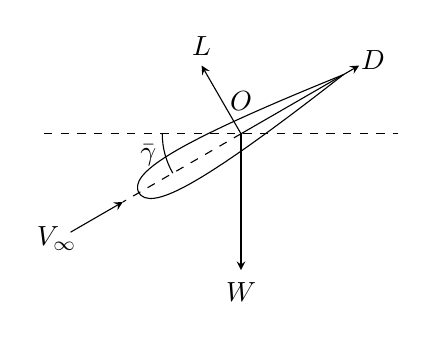
\begin{tikzpicture}[>=stealth]
  % The origin
  \coordinate [label={[xshift=0pt, yshift=5pt] $O$}] (O) at (0.0, 0.0);
  % Weight
  \coordinate [label={[xshift=0pt, yshift=-15pt] $W$}] (W) at (-90:3^0.5);
  % Drag
  \coordinate [label={[xshift=5pt, yshift=-5pt] $D$}] (D) at (30:3^0.5);
  % Lift
  \coordinate [label={[xshift=0pt, yshift=0pt] $L$}] (L) at (120:1);
    
  % The leading edge
  \coordinate (le) at (210:1.5);
  % The trailing edge
  \coordinate (te) at (30:1.5);
  % The left side of the horizontal rule
  \coordinate (hl) at (-2.5,0.0);
  % The right side of the horizontal rule
  \coordinate (hr) at (2.0,0.0);

  % Freestream velocity
  \coordinate [label={[xshift=-5pt, yshift=-10pt] $V_{\infty}$}] (V) at (210:2.5);
  % Another point of the velocity
  \coordinate (v) at (210:3^0.5);

  % The starting point of the flight path angle gamma
  \coordinate [label={[xshift=-5pt, yshift=-15pt] $\bar{\gamma}$}] (g) at (-1.0, 0.0);

  % Forces
  \draw [->] (O) -- (W);
  \draw [->] (O) -- (D);
  \draw [->] (O) -- (L);

  % Chord line
  \draw [dashed] (O) -- (v);

  % The airfoil
  \draw (le) .. controls (200:1.5) and  (190:1.0) .. (te);
  \draw (le) .. controls (220:1.5) and  (230:1.0) .. (te);

  % The horizontal rule
  \draw [dashed] (hl) -- (hr);

  % Freestream velocity
  \draw [->] (V) -- (v);

  % The flight path angle
  \draw (g) arc [start angle=180, end angle=210, radius=1.0];
  \end{tikzpicture}
  
  \caption{The free body diagram of a poweroff glide}
  \label{fig:fbd}
\end{figure}
Also, the relations between speeds are given in Figure \ref{fig:velocities}, note that a positive $V_{\text{wind}}$ represents a tailwind.
\begin{figure}[!htp]
  \centering

  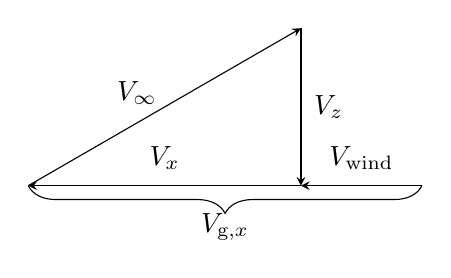
\begin{tikzpicture}[>=stealth]
  \coordinate (a) at (0.0, 0.0);
  \coordinate (b) at (2*3^0.5, 2.0);
  \coordinate (c) at (2*3^0.5, 0.0);
  \coordinate (d) at (5.0, 0.0);
  
  \path [->] (a) edge node [xshift=-10pt, yshift=5pt]{$V_{\infty}$} (b);
  \path [->] (b) edge node [xshift=10pt, yshift=0pt]{$V_{z}$} (c);
  \path [->] (c) edge node [xshift=0pt, yshift=10pt]{$V_{x}$} (a);
  \path [->] (d) edge node [xshift=0pt, yshift=10pt]{$V_{\text{wind}}$} (c);
  \draw [decorate,decoration={brace,amplitude=10pt,mirror}] (a) -- (d) node[midway,yshift=-15pt] {$V_{\text{g}, x}$};
  \end{tikzpicture}
  
  \caption{The relations between speeds}
  \label{fig:velocities}
\end{figure}

Then we have
\[\begin{aligned}
V_{x} & = V_{\infty} \cos \bar{\gamma} = V_{\infty} \frac{L}{W}, \cr
V_{z} & = V_{\infty} \sin \bar{\gamma} = V_{\infty} \frac{D}{W}. \cr
\end{aligned}\]
And by definition, the endurance $E$ is
\[
E = \frac{H}{V_{z}} = \frac{H}{V_{\infty} \frac{D}{W}} = \frac{HW}{V_{\infty} D},
\]
and the range $R$ is
\[\begin{aligned}
R = E V_{\text{g}, x}
& = \frac{HW}{V_{\infty} D} V_{\text{g}, x} \cr
& = \frac{HW}{D} \frac{V_{\text{g}, x}}{(V_{\text{g}, x} - V_{\text{wind}}) \frac{W}{L}} \cr
& = H \frac{L}{D} \frac{V_{\text{g}, x}}{V_{\text{g}, x} - V_{\text{wind}}} \cr
& = H \frac{C_{L}}{C_{D}} \frac{V_{\text{g}, x}}{V_{\text{g}, x} - V_{\text{wind}}},
\end{aligned}\]
which implies a positive $V_{\text{wind}}$, or a tailwind increases the range, if $V_{\text{g}, x}$ is a constant.
\end{document}